\begin{frame}
	\myheading{Module 2.2: McCulloch Pitts Neuron}
\end{frame}


\begin{frame}
	\begin{columns}
		\column{0.4\textwidth}
		\begin{overlayarea}{\textwidth}{\textheight}
			\begin{figure}
				\begin{tikzpicture}
	\node[name=s,shape=circle split,draw=gray!40,line width=0mm,minimum size=2cm] {};

	\begin{scope}[on background layer]
		\fill[black!50] (s.base) ([xshift=-0mm]s.east) arc (0:180:1cm-0mm)--cycle;
		\fill[white!50] (s.base) ([xshift=0mm]s.west) arc (180:360:1cm-0mm)--cycle;
	\end{scope}

	\onslide<2->{\node (input0) at (-1.5, -2.0) {$x_1$};}
	\onslide<3->{\node (input1) at (-0.75, -2.0) {$x_2$};}
	\onslide<4->{\node (input2) at (0, -2.0) {$..$};}
	\onslide<4->{\node (input3) at (0.75, -2.0) {$..$};}
	\onslide<5->{\node (input4) at (2.25, -2.0) {$x_n \onslide<6->{\in \{0,1\}}$};}

	\onslide<9->{\node (output) at (0, 2.0) {$y \in \{0,1\}$};}

	\onslide<7->{\node at (0,-0.5) {$g$};}
	\onslide<8->{\node at (0,0.5) {$f$};}

	\draw [->] (input0) -- (s.240);
	\draw [->] (input1) -- (s.255);
	\draw [->] (input2) -- (s.270);
	\draw [->] (input3) -- (s.285);
	\draw [->] (input4) -- (s.300);
	\draw [->] (s.90) -- (output);

\end{tikzpicture}
				%\caption{A generic computing unit}
			\end{figure}

		\end{overlayarea}
		\column{0.6\textwidth}
		\begin{overlayarea}{\textwidth}{\textheight}
			\begin{itemize}\justifying
				\item McCulloch (neuroscientist) and Pitts (logician) proposed a highly simplified computational model of the neuron (1943)
				\item<7-> $g$ aggregates the inputs \onslide<8->{and the function $f$ takes a decision based on this aggregation}
				\item<10-> The inputs can be excitatory or inhibitory
				\item<11-> $y = 0$ if any $x_i$ is inhibitory, else

				      \onslide<12->{
					      \begin{align*}
						      \onslide<12->{g(x_1, x_2, ..., x_n) & = g(\mathbf{x}) = \sum_{i=1}^{n} x_i \\}
						      \onslide<13->{y = f (g(\mathbf{x})) & = 1 \quad if \quad g(\mathbf{x}) \geq \theta \\}
						      \onslide<14->{                      & = 0 \quad if \quad g(\mathbf{x}) < \theta}
					      \end{align*}
				      }

				      \vspace{-0.4in}
				\item<15-> $\mathbf{\theta}$ is called the thresholding parameter
				\item<16-> This is called Thresholding Logic
			\end{itemize}
		\end{overlayarea}
	\end{columns}
\end{frame}

\begin{frame}
	Let us implement some boolean functions using this McCulloch Pitts (MP) neuron ...
\end{frame}


\begin{frame}
	\begin{columns}
		\column{0.33\textwidth}
		\begin{overlayarea}{\textwidth}{\textheight}
			\begin{center}
				\begin{tikzpicture}
	\node[name=s,shape=circle split,draw=gray!40,line width=0mm,minimum size=1cm] {};
	\begin{scope}[on background layer]
		\fill[black!50] (s.base) ([xshift=-0mm]s.east) arc (0:180:0.5cm-0mm)--cycle;
		\fill[white!50] (s.base) ([xshift=0mm]s.west) arc (180:360:0.5cm-0mm)--cycle;
	\end{scope}
	\node (input1) at (-0.75, -1.25) {$x_1$};
	\node (input2) at (0, -1.25) {$x_2$};
	\node (input3) at (0.75, -1.25) {$x_3$};

	\node (output) at (0, 1.25) {$y \in \{0,1\}$};

	%\node at (0,0.25) {$f$};
	\node at (0,-0.25) {$\theta$};

	\draw [->] (input1) -- (s.255);
	\draw [->] (input2) -- (s.270);
	\draw [->] (input3) -- (s.285);
	\draw [->] (s.90) -- (output);

\end{tikzpicture}
				\captionof{figure}{A McCulloch Pitts unit}

				\only<6->{
					\begin{tikzpicture}
	\node[name=s,shape=circle split,draw=gray!40,line width=0mm,minimum size=1cm] {};
	\begin{scope}[on background layer]
		\fill[black!50] (s.base) ([xshift=-0mm]s.east) arc (0:180:0.5cm-0mm)--cycle;
		\fill[white!50] (s.base) ([xshift=0mm]s.west) arc (180:360:0.5cm-0mm)--cycle;
	\end{scope}
	\node (input1) at (-0.75, -1.25) {$x_1$};
	\node (input2) at (0.75, -1.25) {$x_2$};

	\node (output) at (0, 1.25) {$y \in \{0,1\}$};

	%\node at (0,0.25) {$f$};
	\onslide<7->{\node at (0,-0.25) {$1$};}

	\draw [->] (input1) -- (s.255);
	\draw [o=1pt] (input2) -- (s.285);
	\draw [->] (s.90) -- (output);

\end{tikzpicture}
					\captionof{figure}{$x_1$ AND $!x_2$$^*$ \footnotetext{$^*$circle at the end indicates inhibitory input: if any inhibitory input is 1 the output will be 0}}
				}
			\end{center}

		\end{overlayarea}

		\column{0.33\textwidth}
		\begin{overlayarea}{\textwidth}{\textheight}
			\begin{center}
				\only<2->{
					\begin{tikzpicture}
	\node[name=s,shape=circle split,draw=gray!40,line width=0mm,minimum size=1cm] {};
	\begin{scope}[on background layer]
		\fill[black!50] (s.base) ([xshift=-0mm]s.east) arc (0:180:0.5cm-0mm)--cycle;
		\fill[white!50] (s.base) ([xshift=0mm]s.west) arc (180:360:0.5cm-0mm)--cycle;
	\end{scope}
	\node (input1) at (-0.75, -1.25) {$x_1$};
	\node (input2) at (0, -1.25) {$x_2$};
	\node (input3) at (0.75, -1.25) {$x_3$};

	\node (output) at (0, 1.25) {$y \in \{0,1\}$};

	%\node at (0,0.25) {$f$};
	\onslide<3->{\node at (0,-0.25) {3};}

	\draw [->] (input1) -- (s.255);
	\draw [->] (input2) -- (s.270);
	\draw [->] (input3) -- (s.285);
	\draw [->] (s.90) -- (output);

\end{tikzpicture}
					\captionof{figure}{AND function}
				}
				\only<8->{
					\begin{tikzpicture}
	\node[name=s,shape=circle split,draw=gray!40,line width=0mm,minimum size=1cm] {};
	\begin{scope}[on background layer]
		\fill[black!50] (s.base) ([xshift=-0mm]s.east) arc (0:180:0.5cm-0mm)--cycle;
		\fill[white!50] (s.base) ([xshift=0mm]s.west) arc (180:360:0.5cm-0mm)--cycle;
	\end{scope}
	\node (input1) at (-0.75, -1.25) {$x_1$};
	\node (input2) at (0.75, -1.25) {$x_2$};

	\node (output) at (0, 1.25) {$y \in \{0,1\}$};

	%\node at (0,0.25) {$f$};
	\onslide<9->{\node at (0,-0.25) {$0$};}

	\draw [o=1pt] (input1) -- (s.255);
	\draw [o=1pt] (input2) -- (s.285);
	\draw [->] (s.90) -- (output);

\end{tikzpicture}

					\captionof{figure}{NOR function}
				}
			\end{center}
		\end{overlayarea}

		\column{0.33\textwidth}
		\begin{overlayarea}{\textwidth}{\textheight}
			\begin{center}
				\only<4->{
					\begin{tikzpicture}
	\node[name=s,shape=circle split,draw=gray!40,line width=0mm,minimum size=1cm] {};
	\begin{scope}[on background layer]
		\fill[black!50] (s.base) ([xshift=-0mm]s.east) arc (0:180:0.5cm-0mm)--cycle;
		\fill[white!50] (s.base) ([xshift=0mm]s.west) arc (180:360:0.5cm-0mm)--cycle;
	\end{scope}
	\node (input1) at (-0.75, -1.25) {$x_1$};
	\node (input2) at (0, -1.25) {$x_2$};
	\node (input3) at (0.75, -1.25) {$x_3$};

	\node (output) at (0, 1.25) {$y \in \{0,1\}$};

	%\node at (0,0.25) {$f$};
	\onslide<5->{\node at (0,-0.25) {$1$};}

	\draw [->] (input1) -- (s.255);
	\draw [->] (input2) -- (s.270);
	\draw [->] (input3) -- (s.285);
	\draw [->] (s.90) -- (output);

\end{tikzpicture}


					\captionof{figure}{OR function}
				}

				\only<10->{
					\begin{tikzpicture}
	\node[name=s,shape=circle split,draw=gray!40,line width=0mm,minimum size=1cm] {};
	\begin{scope}[on background layer]
		\fill[black!50] (s.base) ([xshift=-0mm]s.east) arc (0:180:0.5cm-0mm)--cycle;
		\fill[white!50] (s.base) ([xshift=0mm]s.west) arc (180:360:0.5cm-0mm)--cycle;
	\end{scope}
	\node (input1) at (0.0, -1.25) {$x_1$};
	%\node (input2) at (0.75, -1.25) {$x_2$};

	\node (output) at (0, 1.25) {$y \in \{0,1\}$};

	%\node at (0,0.25) {$f$};
	\onslide<11->{\node at (0,-0.25) {$0$};}

	\draw [o=1pt] (input1) -- (s.270);
	%\draw [o=1pt] (input2) -- (s.285);
	\draw [->] (s.90) -- (output);

\end{tikzpicture}
					\captionof{figure}{NOT function}
				}
			\end{center}
		\end{overlayarea}
	\end{columns}
\end{frame}

\begin{frame}
	\begin{itemize}\justifying
		\item Can any boolean function be represented using a McCulloch Pitts unit ?
		\item<2-> Before answering this question let us first see the geometric interpretation of a MP unit ...
	\end{itemize}
\end{frame}


\begin{frame}
	\begin{columns}
		\column{0.4\textwidth}
		\begin{overlayarea}{\textwidth}{\textheight}
			\begin{center}
				\only<1->{
					\begin{tikzpicture}
	\node[name=s,shape=circle split,draw=gray!40,line width=0mm,minimum size=1cm] {};
	\begin{scope}[on background layer]
		\fill[black!50] (s.base) ([xshift=-0mm]s.east) arc (0:180:0.5cm-0mm)--cycle;
		\fill[white!50] (s.base) ([xshift=0mm]s.west) arc (180:360:0.5cm-0mm)--cycle;
	\end{scope}
	\node (input1) at (-0.75, -1.25) {$x_1$};
	\node (input3) at (0.75, -1.25) {$x_2$};

	\node (output) at (0, 1.25) {$y \in \{0,1\}$};

	%\node at (0,0.25) {$f$};
	\node at (0,-0.25) {1};

	\draw [->] (input1) -- (s.255);
	\draw [->] (input3) -- (s.285);
	\draw [->] (s.90) -- (output);

\end{tikzpicture}

					\centering
					\captionof{figure}{OR function \\ $x_1 + x_2 = \sum_{i=1}^{2} x_i \geq 1$ }
				}

				\only<2->{
					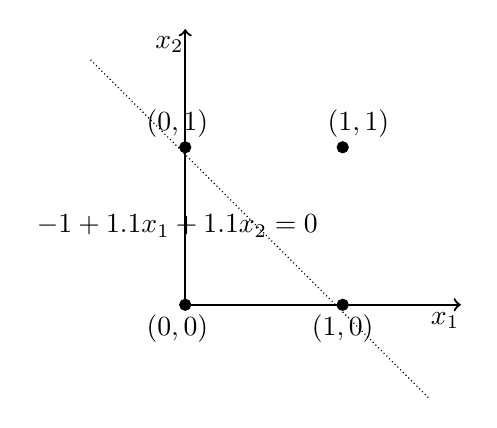
\begin{tikzpicture}
	\draw[thick,->] (0,0) -- (3.5,0);
	\draw[thick,->] (0,0) -- (0,3.5);
	\onslide<16->{\draw[densely dotted] (-1.2021,3.1111) -- (3.1111,-1.2021);}

	\node at (3.3, -0.2) {$x_1$};
	\node at (-0.2, 3.3) {$x_2$};

	\node at (-0.1, -0.3) {$(0,0)$};
	\node at (-0.1, 2.3) {$(0,1)$};
	\node at (2.0, -0.3) {$(1,0)$};
	\node at (2.2, 2.3) {$(1,1)$};
	\onslide<16->{\node at (-0.1, 1.0) {$-1 + 1.1x_1 + 1.1x_2 = 0$};}

	\filldraw (0,0) circle (2pt);
	\filldraw (0,2) circle (2pt);
	\filldraw (2,0) circle (2pt);
	\filldraw (2,2) circle (2pt);
\end{tikzpicture}
				}
			\end{center}
		\end{overlayarea}
		\column{0.6\textwidth}
		\begin{overlayarea}{\textwidth}{\textheight}
			\begin{itemize}\justifying
				\item<4-> A single MP neuron splits the input points (4 points for 2 binary inputs) into two halves
				\item<5-> Points lying on or above the line $\sum_{i=1}^{n} x_i - \theta = 0$ and points lying below this line
				\item<6-> In other words, all inputs which produce an output 0 will be on one side ($\sum_{i=1}^{n} x_i < \theta$) of the line and all inputs which produce an  output 1 will lie on the other side ($\sum_{i=1}^{n} x_i \geq \theta$) of this line
				\item<7-> Let us convince ourselves about this with a few more examples (if it is not already clear from the math)
			\end{itemize}
		\end{overlayarea}
	\end{columns}
\end{frame}


\begin{frame}
	\begin{columns}
		\column{0.4\textwidth}
		\begin{overlayarea}{\textwidth}{\textheight}
			\begin{center}
				\only<1->{
					\begin{tikzpicture}
	\node[name=s,shape=circle split,draw=gray!40,line width=0mm,minimum size=1cm] {};
	\begin{scope}[on background layer]
		\fill[black!50] (s.base) ([xshift=-0mm]s.east) arc (0:180:0.5cm-0mm)--cycle;
		\fill[white!50] (s.base) ([xshift=0mm]s.west) arc (180:360:0.5cm-0mm)--cycle;
	\end{scope}
	\node (input1) at (-0.75, -1.25) {$x_1$};
	\node (input3) at (0.75, -1.25) {$x_2$};

	\node (output) at (0, 1.25) {$y \in \{0,1\}$};

	%\node at (0,0.25) {$f$};
	\node at (0,-0.25) {2};

	\draw [->] (input1) -- (s.255);
	\draw [->] (input3) -- (s.285);
	\draw [->] (s.90) -- (output);

\end{tikzpicture}
					\captionof{figure}{AND function \\ $x_1 + x_2 = \sum_{i=1}^{2} x_i \geq 2$ }
				}
				\only<2->{
					\vspace{-0.2in}
					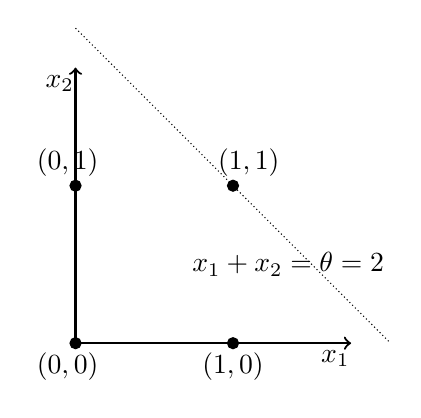
\begin{tikzpicture}

	\draw[thick,->] (0,0) -- (3.5,0);
	\draw[thick,->] (0,0) -- (0,3.5);

	\onslide<3->{\draw[densely dotted] (0.0,4.0) -- (4,0);}

	\node at (3.3, -0.2) {$x_1$};
	\node at (-0.2, 3.3) {$x_2$};

	\node at (-0.1, -0.3) {$(0,0)$};
	\node at (-0.1, 2.3) {$(0,1)$};
	\node at (2.0, -0.3) {$(1,0)$};
	\node at (2.2, 2.3) {$(1,1)$};
	\onslide<3->{\node at (2.7, 1.0) {$x_1 + x_2 = \theta = 2$};}

	\filldraw (0,0) circle (2pt);
	\filldraw (0,2) circle (2pt);
	\filldraw (2,0) circle (2pt);
	\filldraw (2,2) circle (2pt);
\end{tikzpicture}
				}
			\end{center}
		\end{overlayarea}
		\column{0.6\textwidth}
		\begin{overlayarea}{\textwidth}{\textheight}
			\begin{center}
				\only<4->{
					\begin{tikzpicture}
	\node[name=s,shape=circle split,draw=gray!40,line width=0mm,minimum size=1cm] {};
	\begin{scope}[on background layer]
		\fill[black!50] (s.base) ([xshift=-0mm]s.east) arc (0:180:0.5cm-0mm)--cycle;
		\fill[white!50] (s.base) ([xshift=0mm]s.west) arc (180:360:0.5cm-0mm)--cycle;
	\end{scope}
	\node (input1) at (-0.75, -1.25) {$x_1$};
	\node (input3) at (0.75, -1.25) {$x_2$};

	\node (output) at (0, 1.25) {$y \in \{0,1\}$};

	%\node at (0,0.25) {$f$};
	\only<5->{\node at (0,-0.25) {0};}

	\draw [->] (input1) -- (s.255);
	\draw [->] (input3) -- (s.285);
	\draw [->] (s.90) -- (output);

\end{tikzpicture}
					\captionof{figure}{Tautology (always ON)}
				}

				\only<6->{
					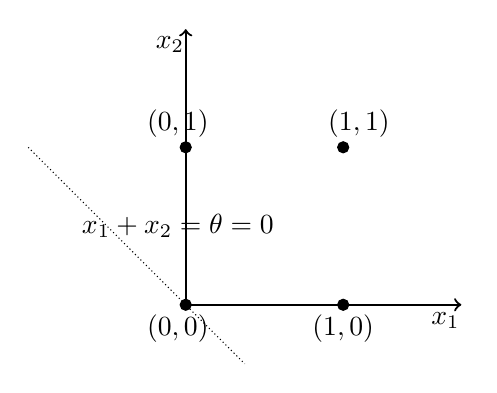
\begin{tikzpicture}

	\draw[thick,->] (0,0) -- (3.5,0);
	\draw[thick,->] (0,0) -- (0,3.5);

	\onslide<7->{\draw[densely dotted] (-2.0,2.0) -- (0.75,-0.75);}

	\node at (3.3, -0.2) {$x_1$};
	\node at (-0.2, 3.3) {$x_2$};

	\node at (-0.1, -0.3) {$(0,0)$};
	\node at (-0.1, 2.3) {$(0,1)$};
	\node at (2.0, -0.3) {$(1,0)$};
	\node at (2.2, 2.3) {$(1,1)$};
	\onslide<7->{\node at (-0.1, 1.0) {$x_1 + x_2 = \theta = 0$};}

	\filldraw (0,0) circle (2pt);
	\filldraw (0,2) circle (2pt);
	\filldraw (2,0) circle (2pt);
	\filldraw (2,2) circle (2pt);
\end{tikzpicture}
				}
			\end{center}
		\end{overlayarea}
	\end{columns}
\end{frame}


\begin{frame}
	\begin{columns}
		\column{0.5\textwidth}
		\begin{overlayarea}{\textwidth}{\textheight}
			\begin{center}
				
\begin{tikzpicture}
	\node[name=s,shape=circle split,draw=gray!40,line width=0mm,minimum size=1cm] {};
	\begin{scope}[on background layer]
		\fill[black!50] (s.base) ([xshift=-0mm]s.east) arc (0:180:0.5cm-0mm)--cycle;
		\fill[white!50] (s.base) ([xshift=0mm]s.west) arc (180:360:0.5cm-0mm)--cycle;
	\end{scope}
	\node (input1) at (-0.75, -1.25) {$x_1$};
	\node (input2) at (0.0, -1.25) {$x_2$};
	\node (input3) at (0.75, -1.25) {$x_3$};

	\node (output) at (0, 1.25) {$y \in \{0,1\}$};

	%\node at (0,0.25) {$f$};
	\node at (1.5,-0.25) {OR};

	\node at (0,-0.25) {1};

	\draw [->] (input1) -- (s.255);
	\draw [->] (input2) -- (s.270);
	\draw [->] (input3) -- (s.285);
	\draw [->] (s.90) -- (output);
\end{tikzpicture}

				\only<2->{
					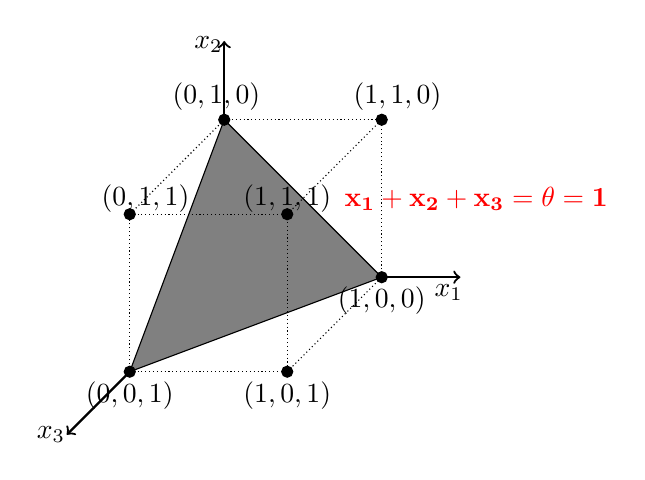
\begin{tikzpicture}

	\draw[thick,->] (0,0) -- (3.0,0);
	\draw[thick,->] (0,0) -- (0,3.0);
	\draw[thick,->] (0,0) -- (-2.0,-2.0);


	\node at (2.85, -0.2) {$x_1$};
	\node at (-0.2, 2.95) {$x_2$};
	\node at (-2.2, -2.0) {$x_3$};

	\node at (-0.1, -0.3) {$(0,0,0)$};
	\filldraw[fill=red] (0,0) circle (2pt);

	\only<5->{\draw[black, fill=gray] (2,0) -- (0,2) -- (-1.2,-1.2) -- (2,0) -- cycle;}

	\node at (-0.1, 2.3) {$(0,1,0)$};
	\node at (2.0, -0.3) {$(1,0,0)$};
	\node at (2.2, 2.3) {$(1,1,0)$};
	\node at (-1.2,-1.5) {$(0,0,1)$};
	\node at (0.8,-1.5) {$(1,0,1)$};
	\node at (-1.0,1.0) {$(0,1,1)$};
	\node at (0.8,1.0) {$(1,1,1)$};
	\onslide<5->{\node at (3.2, 1.0) {\color{red}{$\mathbf{x_1 + x_2 + x_3 = \mathbf{\theta} = 1}$}};}

	\filldraw (0,2) circle (2pt);
	\filldraw (2,0) circle (2pt);
	\filldraw (2,2) circle (2pt);
	\filldraw (-1.2,-1.2) circle (2pt);
	\filldraw (-1.2,0.8) circle (2pt);
	\filldraw (0.8,-1.2) circle (2pt);


	\draw[densely dotted] (0, 2) -- (-1.2,0.8);
	\draw[densely dotted] (-1.2,-1.2) -- (-1.2,0.8);
	\draw[densely dotted] (0.0,2.0) -- (2,2);
	\draw[densely dotted] (2.0,0.0) -- (2,2);
	\draw[densely dotted] (0.8,0.8) -- (2,2);
	\draw[densely dotted] (0.8,0.8) -- (0.8,-1.2);
	\draw[densely dotted] (0.8,-1.2) -- (2,0);
	\draw[densely dotted] (-1.2,-1.2) -- (0.8,-1.2);
	\draw[densely dotted] (-1.2,0.8) -- (0.8,0.8);


	\filldraw (0.8,0.8) circle (2pt);

\end{tikzpicture}
				}
			\end{center}
		\end{overlayarea}

		\column{0.5\textwidth}
		\begin{overlayarea}{\textwidth}{\textheight}
			\begin{itemize}\justifying
				\item<1-> What if we have more than 2 inputs?
				\item<3-> Well, instead of a line we will have a plane
				\item<4-> For the OR function, we want a plane such that the point (0,0,0) lies on one side and the remaining 7 points lie on the other side of the plane

			\end{itemize}
		\end{overlayarea}
	\end{columns}
\end{frame}


\begin{frame}
	\begin{block}{The story so far ...}
		\onslide<1->{
			\begin{itemize}\justifying
				\item<1-> A single McCulloch Pitts Neuron can be used to represent boolean functions which are linearly separable
				\item<2-> Linear separability (for boolean functions) : There exists a line (plane) such that all inputs which produce a 1 lie on one side of the line (plane) and all inputs which produce a 0 lie on other side of the line (plane)
			\end{itemize}
		}
	\end{block}
\end{frame}
